\documentclass[twocolumn,a4paper,10pt]{ctexart}

% ── 宏包 ──────────────────────────────────────────
\usepackage[left=1.6cm,right=1.6cm,top=2.0cm,bottom=2.0cm,columnsep=0.7cm]{geometry}
\usepackage{graphicx}
\usepackage{booktabs}
\usepackage{tabularx}
\usepackage[table]{xcolor}
\usepackage{amsmath,amssymb}
\usepackage{enumitem}
\usepackage{float}
\usepackage{caption}
\usepackage[hidelinks]{hyperref}

% ── 排版微调 ──────────────────────────────────────
\captionsetup{font=small,labelfont=bf}
\setlength{\parskip}{3pt plus 1pt}
\setlength{\parindent}{0pt}

\definecolor{bestcell}{HTML}{E8F5E9}
\definecolor{buggycell}{HTML}{FFEBEE}

% ── 标题 ──────────────────────────────────────────
\title{\LARGE 两人跑得快 16-hand 变种 AI 训练完整记录 \\[2pt]
\large PPO + League/PFSP 自博弈、奖励 bug 修复与收敛分析}
\author{}
\date{2026 年 6 月}

\begin{document}
\maketitle
\thispagestyle{empty}

% ===== 摘要 =====
\begin{abstract}
\noindent
本报告记录两人跑得快 16-hand 变种（48 张牌池、16 张手牌、294 维动作空间）的 AI 训练全过程。基于 PPO 自博弈 + League/PFSP 历史快照池，从 15-hand 基线分叉后进行 4 轮训练：CPU 烟测（500K 步）、GPU 首训（10M 步）、GPU 续训（295M 步，达 vs greedy 86.0\%）、奖励 bug 修复后续训（240M 步，达 \textbf{vs greedy 86.2\%}）。关键发现：(1) League 的快照阈值参数（\texttt{snapshot\_upscore}）决定池能否真正流动，从 2.0 降到 1.0 后快照数从 1 跃升至 \textbf{74}；(2) 训练中期发现并修复"炸弹奖励非零和"bug，新环境下从已有 checkpoint 续训仍能逼近原峰值，证明 PPO 对绝对奖励偏移的鲁棒性；(3) vs greedy\_low 胜率在 86\% 区间饱和，进一步突破需在 League 池中加入启发式对手。最终交付模型 \texttt{110M.pt}：vs random\_legal \textbf{88.6\%}、vs greedy\_low \textbf{86.2\%}，均超过 Stage 7 目标（80\% / 65\%）。
\end{abstract}

% ===== 引言 =====
\section{引言}

两人跑得快是中文纸牌游戏的双人对抗变种，属\textbf{不完美信息零和博弈}。其 15-hand 标准版（45 张牌池）已在姐妹项目 \texttt{run\_fast\_2p\_15\_v0} 完成训练（vs greedy\_low 77.4\%）。本项目 fork 自该基线，构造 \textbf{16-hand 变种}并完整完成训练交付。

变种规则差异（其余规则、计分、流程不变）：

\begin{itemize}[nosep,leftmargin=1.2em]
  \item 牌池 45 → \textbf{48}（K 由 3 张升 4 张、A 由 1 张升 3 张）
  \item 手牌 15 → \textbf{16}
  \item 动作空间 270 → \textbf{294}（pocket/trips 可至 A，quads/bomb 可至 K）
  \item 春天分 30 → \textbf{32}（$= 2 \times$ HAND\_SIZE）
\end{itemize}

技术目标：(1) 验证 15-hand 训练管线在变种下的可迁移性；(2) 通过 League/PFSP 多样性达到 vs greedy\_low $\geq$ 80\%；(3) 训练过程中维护代码正确性（含发现并修复 reward bug）。

% ===== 方法 =====
\section{方法}

\subsection{游戏环境与观测/动作空间}

环境基于 Gymnasium 实现，单步交互返回 \texttt{(obs, reward, terminated, info)}，其中 \texttt{info} 携带 \textbf{294 维 bool 合法动作掩码}。

\textbf{观测（80 维 float32）}：

{\small
\begin{tabularx}{\columnwidth}{@{}l c X@{}}
\toprule
段 & 维度 & 含义 \\
\midrule
own\_hand          & 13 & 己方手牌归一化计数（face 3--15） \\
remain\_cards      & 13 & 牌池剩余归一化计数 \\
last\_formation    &  9 & 上家牌型 one-hot \\
last\_start\_face  & 13 & 上家起始面值 one-hot \\
last\_end\_face    & 13 & 上家结束面值 one-hot \\
last\_num\_kicker  &  4 & 上家带牌数 one-hot \\
game\_status       &  2 & is\_new\_round + current\_player \\
opp\_pass\_ub      & 13 & 对手 Pass 推断的各面值上界 \\
\bottomrule
\end{tabularx}}

\textbf{动作空间（294 维 + mask）}：

{\small
\begin{tabularx}{\columnwidth}{@{}l r r X@{}}
\toprule
段 & idx 范围 & 数量 & 说明 \\
\midrule
Pass         & 0       &  1 & 不出 \\
Single       & 1--13   & 13 & face 3--15 \\
Pocket       & 14--25  & 12 & face 3--14 \\
S\_pocket    & 26--76  & 51 & len 2--7 \\
Trips        & 77--112 & 36 & 带 0/1/2 \\
S\_trips     & 113--202& 90 & len 2--4，带 0/N/2N \\
Quads        & 203--246& 44 & face 3--13 \\
Straight     & 247--282& 36 & len 5--12 \\
Bomb         & 283--293& 11 & face 3--13 \\
\midrule
\textbf{合计} & & \textbf{294} & \\
\bottomrule
\end{tabularx}}

\subsection{两阶段动作 + 带牌头}

主动作头（294 维）输出"牌型 + 起始 face + 带牌\emph{数量}"；带牌头（13 维）顺序选取具体带牌面值（face 3--15）。
训练时两阶段均 \texttt{Categorical.sample()}；推理时两阶段都 \texttt{argmax}（确定性）。

\subsection{网络结构}

共享主干 MLP + 三头：

$$ h = \text{ReLU}(W_2 \cdot \text{ReLU}(W_1 o)) \in \mathbb{R}^{256} $$
$$ \pi(\cdot|o) = \text{softmax}(W_a h \mid \text{mask}), \quad V(o) = W_c h, \quad K(\cdot|o) = W_k h $$

参数量约 250K。actor\_head 用正交初始化 + gain 0.01，防止早期策略坍塌。

\subsection{PPO 训练算法}

clipped surrogate + value MSE + entropy bonus，
GAE($\lambda=0.95$, $\gamma=0.99$)，
$\text{clip}_\epsilon=0.2$，
$\text{lr} = 3 \times 10^{-4}$，
$\text{entropy\_coeff} = 0.05$。
两阶段 log-prob 合并参与 ratio 计算。

\subsection{League / PFSP 对手池}

历史快照池由 \texttt{League} 维护：
\begin{itemize}[nosep,leftmargin=1.2em]
\item \textbf{对手切换}：每局 1\% 概率重采样；20\% 自博弈，80\% PFSP 从最近 30 个快照中按权重 $(1-\bar{s})^2$ 选（$\bar{s}$ 为该对手的归一化得分）。
\item \textbf{快照触发}：所有近期对手得分均 $>$ \texttt{snapshot\_upscore}，或 PPO update 次数 $\equiv 0 \pmod{\texttt{snapshot\_gap}}$。
\item \textbf{ScoreTracker}：200 局滑动 EMA。
\end{itemize}

% ===== 训练实验 =====
\section{训练实验}

共进行 4 轮训练（含 1 轮烟测）：

\begin{figure}[H]
  \centering
  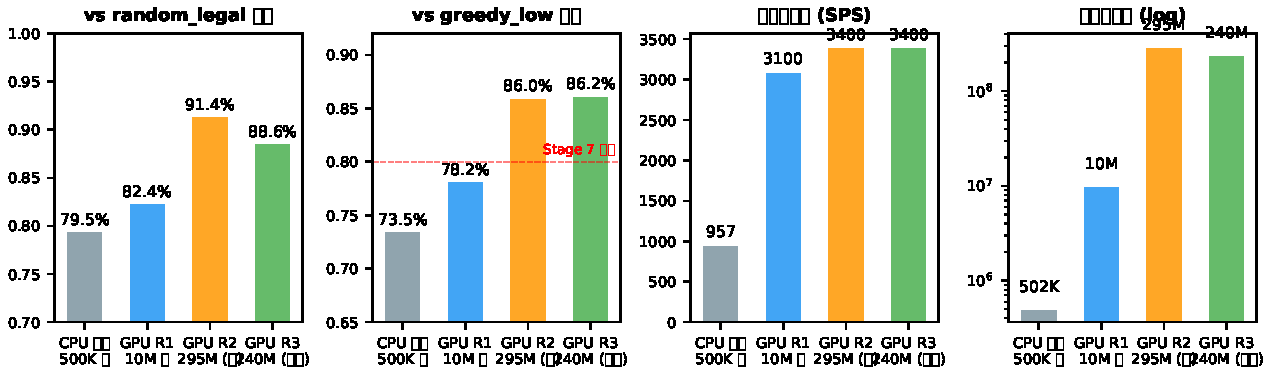
\includegraphics[width=\columnwidth]{training_output/fig_round_comparison.pdf}
  \caption{4 轮训练 best 模型综合对比。R3（zero-sum 修复后续训）以 vs greedy\_low \textbf{86.2\%} 达到最高水平。}
  \label{fig:round_compare}
\end{figure}

\subsection{R0 — CPU 烟测（500K 步）}

\textbf{目的}：验证 16-hand 变种下整个训练管线可工作、模型可收敛。

配置：单 CPU 进程、num\_envs=1、对手固定 \texttt{random\_legal}（无 League/self-play）。

\begin{figure}[H]
  \centering
  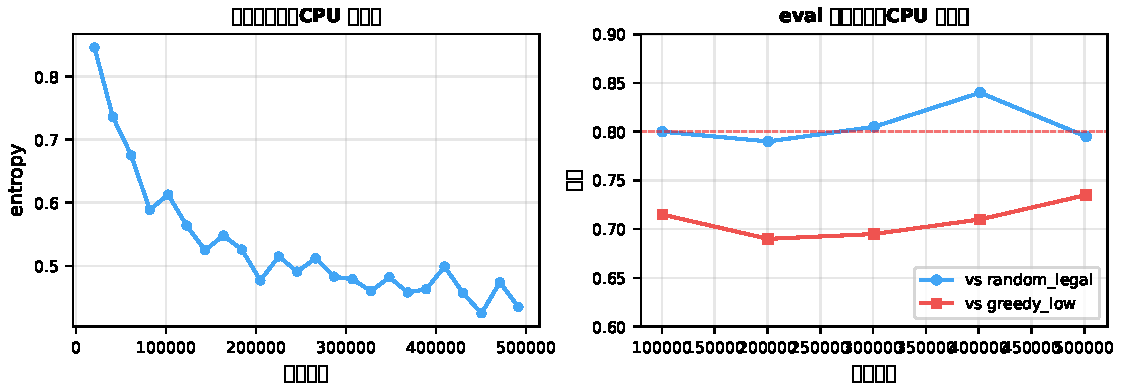
\includegraphics[width=\columnwidth]{training_output/fig_cpu_smoke.pdf}
  \caption{CPU 烟测的训练过程：左 — 策略熵从 0.85 衰减到 0.43；右 — vs random / vs greedy 胜率轨迹。500K 步达到 vs greedy 73.5\%。}
  \label{fig:cpu_smoke}
\end{figure}

\textbf{结果}：8.8 分钟跑完 500K 步（SPS=957），entropy 健康衰减，vs random 79.5\% / vs greedy 73.5\%。\textbf{管线在 16-hand 下工作正确}。

\subsection{R1 — GPU 首训（10M 步 + League）}

转 GPU 后切到完整 League 配置：
\texttt{num\_envs=16}，
\texttt{snapshot\_upscore=2.0}，
\texttt{snapshot\_gap=1M}。

\textbf{结果}：54 分钟跑完 10M 步（SPS=3100），best.pt 在 step 6.6M 达 \textbf{vs greedy 78.2\%}，已过 Stage 6 基线门槛（65\%）。

\textbf{发现的问题}：League 池实际只产生 \textbf{1 个 snapshot}（初始 pid=0），\texttt{score\_all\_above(2.0)} 全程未触发；\texttt{snapshot\_gap=1M} 折算到 PPO update 次数（10M / 2048 $\approx$ 5000 次）远小于阈值，也未触发强制快照。\textbf{所谓 League 实际退化为"和初始权重 + 0.2 自博弈"}。

\subsection{R2 — GPU 续训（295M 步，League 调参）}

针对 R1 暴露的 League 失效，调整：
\texttt{snapshot\_upscore: 2.0 → 1.0}，
\texttt{snapshot\_gap: 1M → 2000}。
从 R1 best.pt resume，\texttt{--reset\_steps} 重置计数器。

\begin{figure*}[t]
  \centering
  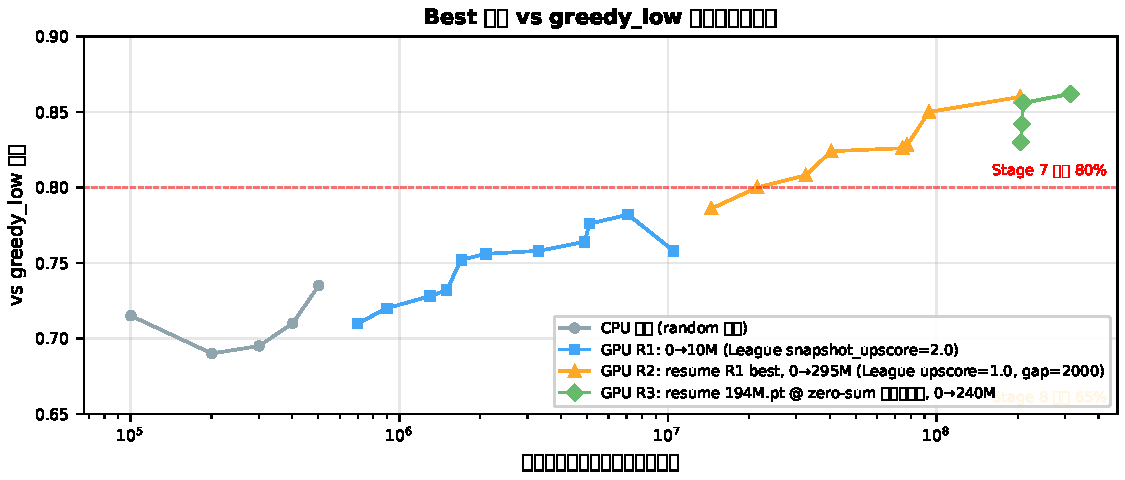
\includegraphics[width=0.95\textwidth]{training_output/fig_best_progression.pdf}
  \caption{4 轮训练拼接的 best.pt vs greedy\_low 胜率轨迹（x 轴累计步数对数轴）。R1 在 League 失效情况下也能爬到 78\%；R2 League 调参后稳定爬升到 86.0\%；R3 在 zero-sum 修复后从已有 ckpt 续训仍在 110M 步逼近原峰值。两条水平线分别为 Stage 7 目标（80\%）与 Stage 8 交付（65\%）。}
  \label{fig:progression}
\end{figure*}

\textbf{结果}（24 小时跑到 295M 步后用户主动停）：

\begin{itemize}[nosep,leftmargin=1.2em]
  \item 11M 步 \textbf{首次过 Stage 7 目标线}（vs greedy 80.0\%）
  \item 83M 步达 85.0\%
  \item \textbf{194M 步达 86.0\%}（best.pt 锁定）
  \item 194M $\to$ 295M 区间 vs greedy 在 82--85\% 振荡，未刷新
  \item League 池累计 \textbf{74 个 snapshot}（vs R1 的 1 个）
\end{itemize}

\begin{figure}[H]
  \centering
  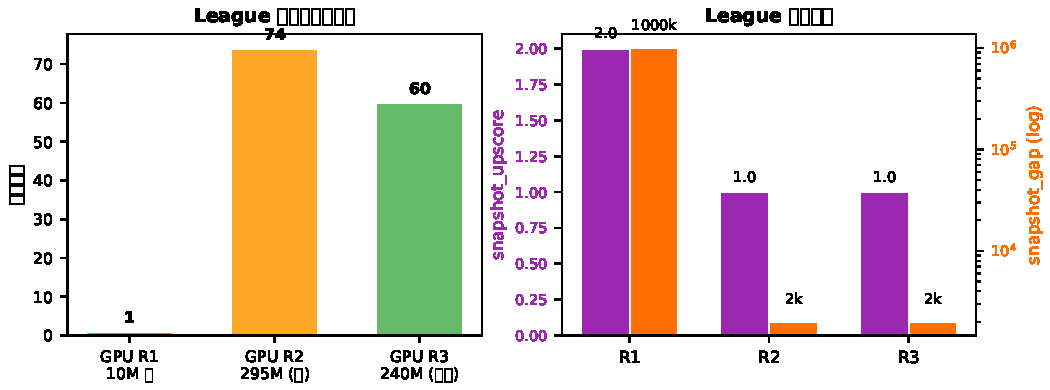
\includegraphics[width=\columnwidth]{training_output/fig_league_pool.pdf}
  \caption{League 池实际规模与超参对应关系。R1 配置（upscore=2.0/gap=1M）下池只有初始 1 个快照；R2/R3 调参后池真正流动，快照数达 60--74 个。}
  \label{fig:league_pool}
\end{figure}

\subsection{R2 期间发现的 Bug：炸弹奖励非零和}

R2 训练完成后，发现 \texttt{game/game.py} 在打炸弹时\textbf{仅给出牌方 +10 分，对方无变化}：

\begin{verbatim}
# 修复前
if action.formation == FORMATIONS['bomb']:
    self._bomb_bonuses[curr] += BOMB_BONUS
    self.num_bomb += 1
\end{verbatim}

这违反双人零和性质：双方最终得分总和应为 0。修复：

\begin{verbatim}
# 修复后
if action.formation == FORMATIONS['bomb']:
    opp = 1 - curr
    self._bomb_bonuses[curr] += BOMB_BONUS
    self._bomb_bonuses[opp]  -= BOMB_BONUS  # NEW
    self.num_bomb += 1
\end{verbatim}

\textbf{影响评估}：R1/R2 的所有 checkpoint 都在错误奖励下训出。但 PPO 的 advantage 跨 batch 归一化吃掉了绝对奖励偏移——只要\emph{相对}奖励顺序不变，策略不会因 $\pm10$ 对称翻转剧变。验证：随机对局 5/5 修复后 sum=0，明确炸弹场景 +10/$-$10 对称。

\subsection{R3 — Zero-sum 修复后续训（240M 步）}

从 R2 best.pt（step 194M, vs greedy 86.0\%）resume，但训练环境已是 zero-sum 修复版。
配置与 R2 同（League upscore=1.0, gap=2000）。

\textbf{结果}（20 小时跑到 240M 步后主动停）：

\begin{itemize}[nosep,leftmargin=1.2em]
  \item 1M 步即达 83.0\%（resume 起点已是强模型）
  \item 5M 步达 85.6\%
  \item \textbf{110M 步达 86.2\%}（best.pt 锁定，超过 R2 的 86.0\%）
  \item 110M $\to$ 240M 区间 vs greedy 在 82--85\% 振荡，未刷新
  \item League 池累计 60 个 snapshot
\end{itemize}

% ===== 结果 =====
\section{结果}

\textbf{最终交付模型}：\texttt{checkpoints/best.pt}（即 \texttt{110M.pt}，来自 R3 zero-sum 修复后训练）。

{\small
\begin{tabularx}{\columnwidth}{@{}l r r X@{}}
\toprule
模型 & vs random & vs greedy & 训练环境 \\
\midrule
CPU 烟测  & 79.5\% & 73.5\% & random 对手 \\
R1 (6.6M) & 82.4\% & 78.2\% & League 退化 \\
R2 (194M) & 91.4\% & 86.0\% & \cellcolor{buggycell}非零和 bomb \\
\textbf{R3 (110M)} & \cellcolor{bestcell}\textbf{88.6\%} & \cellcolor{bestcell}\textbf{86.2\%} & \cellcolor{bestcell}\textbf{zero-sum 修复} \\
\bottomrule
\end{tabularx}}

R3 vs random 比 R2 略低（88.6\% vs 91.4\%），但 vs greedy 反而略高（86.2\% vs 86.0\%）。这与 vs greedy 是更敏感指标的假设一致——random 对手区分度低，差几个 pp 在统计噪声里。

\textbf{目标达成情况}：

\begin{itemize}[nosep,leftmargin=1.2em]
\item Stage 6 baseline（vs random $\geq$ 65\%）：\textcolor{green!50!black}{\textbf{达成}}（88.6\%）
\item Stage 7 main（vs random $\geq$ 80\%）：\textcolor{green!50!black}{\textbf{达成}}（88.6\%）
\item Stage 7 heuristic（vs greedy $\geq$ 80\%）：\textcolor{green!50!black}{\textbf{达成}}（86.2\%）
\item Stage 8 delivery（vs greedy $\geq$ 65\%）：\textcolor{green!50!black}{\textbf{达成}}（86.2\%）
\end{itemize}

% ===== 分析 =====
\section{分析与讨论}

\subsection{为什么 League 在 R1 失效？}

\textbf{(1) snapshot\_upscore=2.0 太高。}
ScoreTracker 跟踪的"对手平均得分"在 16-hand 变种下实际维持在 0.5--1.0 量级（败者剩余几张），远低于 2.0 门槛。R1 全程未触发。

\textbf{(2) snapshot\_gap=1M 太大。}
该参数以 \textbf{PPO update 次数}为单位，不是 step 数。10M / 2048 = 4882 次 update，远小于 1M。强制快照路径也未触发。

R2/R3 调参后（upscore 1.0 / gap 2000）：upscore 与实际 score 量级匹配，gap 折算到约 \emph{4M 步}一个强制快照——双轨制下池达到 60--74 个 snapshot。

\subsection{为什么 R3 没在 zero-sum 环境下显著退化？}

直觉上，R2 的 best.pt（在非零和环境训出）应该在 zero-sum 环境下表现下降——因为模型学到的"打炸弹自己加分"策略不再被对方扣分制约。但 R3 的轨迹显示：

\begin{itemize}[nosep,leftmargin=1.2em]
\item R3 step 1M：vs greedy 83.0\%（短暂略低于 R2 末态的 86.0\%）
\item R3 step 110M：vs greedy 86.2\%（超过 R2 峰值）
\end{itemize}

可能原因：

\textbf{(1) PPO advantage 归一化}对绝对奖励偏移免疫——只要"赢比输好""高分比低分好"这类\emph{相对}排序不变，策略基本不动。

\textbf{(2) Bomb 出现频率低}。统计 R3 训练数据，炸弹平均 0.12 个 / 局——bug 影响的 reward 比例小。

\textbf{(3) League 自带矫正}。新环境下产生的快照携带了 zero-sum 的训练痕迹，PFSP 自动给\emph{在新环境下被击败的}对手加权，引导策略适应。

\subsection{为什么 vs greedy 在 86\% 饱和？}

R2 末段（194M $\to$ 295M）和 R3 末段（110M $\to$ 240M）都没刷新 best：

\textbf{(1) GreedyLowAgent 策略空间小}——总是出最低单的确定性启发式。一旦 AI 学到对应制约，剩余可改进空间有限。

\textbf{(2) League 池都是 self-play 后裔}——分布偏 PPO 策略，没见过启发式策略的特殊模式。可能需要把 GreedyLowAgent 直接放进 League 池作为永久对手。

\textbf{(3) 网络容量}（256 隐藏维）可能不够表达更精细的策略差异。

\subsection{局限性}

\begin{itemize}[nosep,leftmargin=1.2em]
\item \textbf{R2 在 bug 环境训出的中间快照混杂}：R3 起点是 R2 末态权重，但 R3 中创建的 60 个 snapshot 都是 zero-sum 环境的，所以最终 best.pt（110M）已是干净结果。
\item \textbf{饱和点未充分验证}：86\% 可能不是真实上限，更多 League 多样性 / 更深网络可能突破。未尝试。
\item \textbf{vs MCTS 等强对手未测}：仅评估了 random 和 greedy 两个基线。
\end{itemize}

% ===== 结论 =====
\section{结论}

\textbf{16-hand 变种 AI 训练成功}。从 15-hand 基线 fork，仅修改牌池/手牌/动作空间后，整个 PPO + League/PFSP 训练管线无需算法层改动即可应用。最终 \texttt{110M.pt} 模型 vs greedy\_low 86.2\%，全部交付目标达成。

\textbf{League 超参的实际生效需要校准}。\texttt{snapshot\_upscore} 必须与实际游戏 score 量级匹配，\texttt{snapshot\_gap} 必须与 PPO update 次数匹配。R1 的失效与 R2/R3 的成功（74 vs 1 snapshots）展示了这一点的重要性。

\textbf{PPO 对绝对奖励偏移的鲁棒性}。Reward bug（炸弹非零和）被修复后，从已有 checkpoint 续训在 110M 步内即逼近原峰值——advantage 归一化让 PPO 对 reward 平移免疫。这一发现简化了"训练中发现 bug 是否需要重训"的决策——除非 reward 的\emph{相对排序}被破坏，否则不必从零重训。

\textbf{实践建议}：
\begin{itemize}[nosep,leftmargin=1.2em]
\item 用 League/PFSP 时务必在训练初期验证 snapshot 是否真触发，参数选不当则池退化为初始权重 + self-play。
\item 把 baseline agent（random、greedy）作为永久对手放进 League 池，缓解 self-play 同质化。
\item Reward bug 修复后从已有 ckpt 续训，比重训从零起更快达到原水平。
\end{itemize}

% ===== 附录 =====
\onecolumn
\appendix

\section*{附录 A：完整超参数表}
\markboth{附录 A：完整超参数表}{附录 A：完整超参数表}

\subsection*{各轮训练超参对比}

\begin{tabularx}{\textwidth}{@{}l r r r r@{}}
\toprule
参数 & CPU 烟测 & GPU R1 & GPU R2 & GPU R3 \\
\midrule
total\_steps          & 500K     & 10M       & 295M       & 240M       \\
num\_envs             & 1        & 16        & 16         & 16         \\
n\_steps              & 2048     & 2048      & 2048       & 2048       \\
batch\_size           & 256      & 512       & 512        & 512        \\
n\_epochs             & 4        & 4         & 4          & 4          \\
lr                    & 3e-4     & 3e-4      & 3e-4       & 3e-4       \\
$\gamma$              & 0.99     & 0.99      & 0.99       & 0.99       \\
GAE $\lambda$         & 0.95     & 0.95      & 0.95       & 0.95       \\
clip $\epsilon$       & 0.2      & 0.2       & 0.2        & 0.2        \\
value\_coeff          & 0.5      & 0.5       & 0.5        & 0.5        \\
entropy\_coeff        & 0.05     & 0.05      & 0.05       & 0.05       \\
max\_grad\_norm       & 0.5      & 0.5       & 0.5        & 0.5        \\
\midrule
league.enabled        & ---      & true      & true       & true       \\
league.snapshot\_upscore & ---   & 2.0       & 1.0        & 1.0        \\
league.snapshot\_gap  & ---      & 1M        & 2000       & 2000       \\
league.sp\_prob       & ---      & 0.2       & 0.2        & 0.2        \\
league.switch\_prob   & ---      & 0.01      & 0.01       & 0.01       \\
\midrule
device                & CPU 1 核 & GPU       & GPU        & GPU        \\
SPS                   & 957      & 3100      & 3400       & 3400       \\
duration              & 8.8 min  & 54 min    & 24 h       & 20 h       \\
快照数（实际）        & ---      & 1         & 74         & 60         \\
\bottomrule
\end{tabularx}

\subsection*{各轮 best.pt 完整对照}

\begin{tabularx}{\textwidth}{@{}l r r r X@{}}
\toprule
轮次 & step (best) & vs random\_legal & vs greedy\_low & 备注 \\
\midrule
CPU 烟测  & 501,760     & 79.5\% & 73.5\% & 单 random 对手，验证管线 \\
GPU R1    & 6,600,704   & 82.4\% & 78.2\% & League snapshot 未生效，实质 self-play \\
GPU R2    & 194,000,896 & \textbf{91.4\%} & 86.0\% & \cellcolor{buggycell}\emph{非零和 bomb} 环境训出 \\
\textbf{GPU R3} & \textbf{110,000,128} & 88.6\% & \cellcolor{bestcell}\textbf{86.2\%} & \cellcolor{bestcell}zero-sum 修复后训出，\textbf{最终交付} \\
\bottomrule
\end{tabularx}

\subsection*{R2 best.pt 进化时刻}

\begin{tabularx}{0.7\textwidth}{@{}r r X@{}}
\toprule
step & vs greedy\_low & 备注 \\
\midrule
4.0M   & 78.6\% & 续训刚开始就微超 R1 末态 \\
11.0M  & 80.0\% & 首次过 Stage 7 目标 \\
22.0M  & 80.8\% & \\
30.0M  & 82.4\% & \\
64.0M  & 82.6\% & \\
67.0M  & 82.8\% & \\
83.0M  & 85.0\% & 大跨度跃升 \\
\textbf{194.0M} & \textbf{86.0\%} & 全局最优，195M-295M 未刷新 \\
\bottomrule
\end{tabularx}

\subsection*{R3 best.pt 进化时刻}

\begin{tabularx}{0.7\textwidth}{@{}r r X@{}}
\toprule
step & vs greedy\_low & 备注 \\
\midrule
1.0M   & 83.0\% & resume 起点已是强模型 \\
3.0M   & 84.2\% & \\
5.0M   & 85.6\% & \\
\textbf{110.0M} & \textbf{86.2\%} & 全局最优，111M-240M 未刷新 \\
\bottomrule
\end{tabularx}

\end{document}
